%==============================================================================
% tento soubor pouzijte jako zaklad
% this file should be used as a base for the thesis
% (c) 2008 Michal Bidlo
% E-mail: bidlom AT fit vutbr cz
% Šablonu upravil / template edited by: Ing. Jaroslav Dytrych, dytrych@fit.vutbr.cz
%==============================================================================
% kodovaní: UTF-8 (zmena prikazem iconv, recode nebo cstocs)
% encoding: UTF-8 (you can change it by command iconv, recode or cstocs)
%------------------------------------------------------------------------------
% zpracování / processing: make, make pdf, make clean
%==============================================================================
% Soubory, které je nutné upravit: / Files which have to be edited:
%   projekt-20-literatura-bibliography.bib - literatura / bibliography
%   projekt-01-kapitoly-chapters.tex - obsah práce / the thesis content
%   projekt-30-prilohy-appendices.tex - přílohy / appendices
%==============================================================================
\documentclass[slovak]{fitthesis} 

% bez zadání - pro začátek práce, aby nebyl problém s překladem
%\documentclass[english]{fitthesis} % without assignment - for the work start to avoid compilation problem
%\documentclass[zadani]{fitthesis} % odevzdani do wisu - odkazy jsou barevné
%\documentclass[english,zadani]{fitthesis} % for submission to the IS FIT - links are color
%\documentclass[zadani,print]{fitthesis} % pro tisk - odkazy jsou černé
%\documentclass[english,zadani,print]{fitthesis} % for the print - links are black
% * Je-li prace psana v anglickem jazyce, je zapotrebi u tridy pouzit 
%   parametr english nasledovne:
%   If thesis is written in english, it is necessary to use 
%   parameter english as follows:
%      \documentclass[english]{fitthesis}
% * Je-li prace psana ve slovenskem jazyce, je zapotrebi u tridy pouzit 
%   parametr slovak nasledovne:
%      \documentclass[slovak]{fitthesis}

% Základní balíčky jsou dole v souboru šablony fitthesis.cls
% Basic packages are at the bottom of template file fitthesis.cls
%zde muzeme vlozit vlastni balicky / you can place own packages here

%---rm---------------
\renewcommand{\rmdefault}{lmr}%zavede Latin Modern Roman jako rm / set Latin Modern Roman as rm
%---sf---------------
\renewcommand{\sfdefault}{qhv}%zavede TeX Gyre Heros jako sf
%---tt------------
\renewcommand{\ttdefault}{lmtt}% zavede Latin Modern tt jako tt

% vypne funkci šablony, která automaticky nahrazuje uvozovky,
% aby nebyly prováděny nevhodné náhrady v popisech API apod.
% disables function of the template which replaces quotation marks
% to avoid unnecessary replacements in the API descriptions etc.
\csdoublequotesoff

% =======================================================================
% balíček "hyperref" vytváří klikací odkazy v pdf, pokud tedy použijeme pdflatex
% problém je, že balíček hyperref musí být uveden jako poslední, takže nemůže
% být v šabloně
% "hyperref" package create clickable links in pdf if you are using pdflatex.
% Problem is that this package have to be introduced as the last one so it 
% can not be placed in the template file.
\ifWis
\ifx\pdfoutput\undefined % nejedeme pod pdflatexem / we are not using pdflatex
\else
  \usepackage{color}
  \usepackage[unicode,colorlinks,hyperindex,plainpages=false,pdftex]{hyperref}
  \definecolor{links}{rgb}{0.4,0.5,0}
  \definecolor{anchors}{rgb}{1,0,0}
  \def\AnchorColor{anchors}
  \def\LinkColor{links}
  \def\pdfBorderAttrs{/Border [0 0 0] }  % bez okrajů kolem odkazů / without margins around links
  \pdfcompresslevel=9
\fi
\else % pro tisk budou odkazy, na které se dá klikat, černé / for the print clickable links will be black
\ifx\pdfoutput\undefined % nejedeme pod pdflatexem / we are not using pdflatex
\else
  \usepackage{color}
  \usepackage[unicode,colorlinks,hyperindex,plainpages=false,pdftex,urlcolor=black,linkcolor=black,citecolor=black]{hyperref}
  \definecolor{links}{rgb}{0,0,0}
  \definecolor{anchors}{rgb}{0,0,0}
  \def\AnchorColor{anchors}
  \def\LinkColor{links}
  \def\pdfBorderAttrs{/Border [0 0 0] } % bez okrajů kolem odkazů / without margins around links
  \pdfcompresslevel=9
\fi
\fi
% Řešení problému, kdy klikací odkazy na obrázky vedou za obrázek
% This solves the problems with links which leads after the picture
\usepackage[all]{hypcap}
\usepackage{tikz}
\usepackage{url}
\usepackage{graphicx}
\usepackage{framed}
\usepackage[]{algorithm2e}
\graphicspath{ {obrazky-figures/} }
\usepackage{listings}

\hypersetup{
  colorlinks = true,
  linkcolor  = black
}

% Informace o práci/projektu / Information about the thesis
%---------------------------------------------------------------------------
\projectinfo{
  %Prace / Thesis
  project=SP,            %typ prace BP/SP/DP/DR  / thesis type (SP = term project)
  year=2017,             %rok odevzdání / year of submission
  date=\today,           %datum odevzdani / submission date
  %Nazev prace / thesis title
  title.cs={Forenzní analýza mobilních zařízení},  %nazev prace v cestine ci slovenstine (dle zadani) / thesis title in czech language (according to assignment)
  title.en={Forensic Analysis of Mobile Devices}, %nazev prace v anglictine / thesis title in english
  %Autor / Author
  author={Dávid Bolvanský},   %cele jmeno a prijmeni autora / full name and surname of the author
  author.name={Dávid},   %jmeno autora (pro citaci) / author name (for reference) 
  author.surname={Bolvanský},   %prijmeni autora (pro citaci) / author surname (for reference) 
}

% řeší první/poslední řádek odstavce na předchozí/následující stránce
% solves first/last row of the paragraph on the previous/next page
\clubpenalty=10000
\widowpenalty=10000

\begin{document}
  % Vysazeni titulnich stran / Typesetting of the title pages
  % ----------------------------------------------
  \maketitle
  % Obsah
  % ----------------------------------------------
  % \tableofcontents
  
  % Seznam obrazku a tabulek (pokud prace obsahuje velke mnozstvi obrazku, tak se to hodi)
  % List of figures and list of tables (if the thesis contains a lot of pictures, it is good)
\ifczech
  \renewcommand\listfigurename{Seznam obrázků}
\fi
\ifslovak
  \renewcommand\listfigurename{Zoznam obrázkov}
\fi

  % \listoffigures
\ifczech
  \renewcommand\listtablename{Seznam tabulek}
\fi
\ifslovak
  \renewcommand\listtablename{Zoznam tabuliek}
\fi

  % \listoftables 

  % vynechani stranky v oboustrannem rezimu
  % Skip the page in the two-sided mode
  \iftwoside
    \cleardoublepage
  \fi

  % Text prace / Thesis text
  % ----------------------------------------------
  \newcommand{\qe}[3]{\begin{quotation} \textit{``#1``} \end{quotation} \begin{flushright} - #2\end{flushright} }

\chapter{Forenzná analýza}


\qe{Aplikovanie metodickej sady techník a procedúr potrebných na získanie dôkazov z dodaného počítačového vybavenia, rôznych pamäťových zariadení a digitálnych médii, ktoré môžu byť následne prezentované v koherentnom a zmysluplnom formáte.}{Dr. H.B. Wolfe}

Incidenty v informačnej bezpečnosti sa odohrávajú vo virtuálnom priestore počítačov a počítačových sieti. V ideálnom prípade by sme mali byť schopní zabrániť prípadným útokom, no nie vždy je to možné. Ak už k bezpečnostnému incidentu dôjde, je potrebné zaistiť dôkazy, správne ich vyhodnotiť a na ich základe vyvodiť závery.

Forenzná analýza je jednou z používaných analýz pri vyšetrovaní trestných činov. Cieľom počítačovej forenznej analýzy je príprava získaných materiálov na ďalšie vyšetrovanie. Rieši problematiku kto, ako a kedy uskutočnil nejakú aktivitu súvisiacu s vykonaným trestným činom. Zahŕňa využitie širokého spektra vyšetrovacích technológií a postupov a metód. Slúži ako prostriedok na získanie dôkazov k trestným činom, zneužitie právomocí, porušenie zákona, interných pravidiel alebo smerníc, preukázanie identity osôb, pravosti listín, dát alebo informácií a to ako účastníkom trestného konania tak aj komerčnej sfére. Musí byť vykonávaná podľa prísnych pravidiel aby boli dôkazy prijateľné pre organy činne v trestnom konaní. Počas forenznej analýzy je kľúčové zbieranie digitálneho dôkazového materiálu. Predmetom skúmania nie sú často len samostatné počítače, ale celé počítačové systémy. Výsledkom forenznej analýzy je znalecký alebo technický posudok alebo vyjadrenie, ktorý má v súdnom konaní dôkazovú hodnotu.

\section{Mobilná forenzná analýza}

\qe{Mobilná forenzná analýza je veda zaoberajúca sa obnovou digitálnych dát z mobilných zariadení podľa striktných foreznych pravidiel za pomoci schválených metód.}{National Institute of Standards and Technology
(NIST)}

Získavanie digitálnych dokázov v mobilných forenzných aktivitách zahŕňa fyzické, logické,
a ručné metódy. Fyzické spôsoby získavania dôkazov sa týkajú obnovy binárne reprezentácie internej pamäte mobilných zariadení
a ich ukladania do súborov. Logické spôsoby pracujú s operačným systémom skúmaného mobilného zariadenia za účelom obnovy logických objektov v súborovom systéme. Ručné spôsoby zahŕňajú zobrazovanie dátového obsahu uloženého v mobilnom zariadení, ktoré vyžaduje manuálnu aktivitu s tlačidlami, klávesnicou či dotykovou obrazovkou a môžu byť nahrávané na externú digitálnu kameru. 

Existujúci výskum v oblasti mobilnej forenznej analýzy je možné klasifikovať do nasledovných častí: 1. preskúmanie možností metód získavania dôkazov, 2. vykonávanie podrobných forenzných postupov, 3. vykonávanie hĺbkovej forenznej analýzy mobilných aplikácií alebo mobilných operačných systémov. 

\begin{figure}[h]
	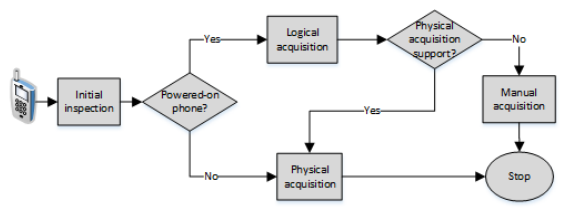
\includegraphics[width=\textwidth]{ziskavanie_dat}
	\caption{Procedúra získavania dát}
\end{figure}


Počiatočná kontrola predstavuje činnosť preskúmania stavu zariadenia zhromažďovaním informácií ako napríklad výrobcu zariadenia, názvu modelu a čísla IMEI. Stav zariadenia rozhoduje o použití techník na získavanie dôkazov. Logické získavanie dôkazov sa vykoná v prípade, že zariadenie je zapnuté. Začína identifikáciou zmeškaných hovorov, neprečítaných správ, času a dátumu pomocou skúmania obrazovky zariadenia. 

Fyzické získavanie dôkazov je vykonávané ak je zariadenie vypnuté. Vykonávanie ručného získavania dôkazov je voliteľné, ak výsledky z logického skúmania sú obmedzené a/alebo fyzické skúmanie nie je podporované. 

\chapter{Terorizmus a mobilné aplikácie}
Mobilné technológie sú často zneužívané na aktivity súvisiace s terorizmom. Forenzná analýza je dôležitý prostriedok pri vyšetrovaní takýchto aktivít. Terorizmus možno definovať ako použitie násilia skupinami alebo jednotlivcami, ktorí sa snažia presadiť svoje politické ciele. Svoje ciele si vyberajú náhodne, často ide o spôsobenie čo najväčších civilných strát.

V nedávnej dobe došlo k incidentu, kedy spoločnosť Apple Inc. odmietla pomôcť Federálnemu vyšetrovaciemu úradu v USA so žiadosťou o odblokovanie šifrovaného iPhone 5C údajne
patriacemu jednému z kľúčových podozrivých, pretože podozrivý deaktivoval iCloud zálohy niekoľko týždňov pred incidentom\footnote{\url{https://assets.documentcloud.org/documents/2716811/Statement-from-the-FBI-Feb-20-2016.pdf}}.

Tento incident si získal znateľný záujem medií, ako aj rozvíril debaty medzi v výskumníkmi a politikmi. Taktiež demonštroval potenciálnu úlohu mobilnej forenznej analýzy pri obnove dôkazových materiálov z mobilných zariadení, ktoré boli použité pri plánovaní, vykonávaní terorizmu a iných kriminálnych aktivít.

Cloudové aplikácie môžu byť používané na ukladanie dát, ktoré môže byť neskôr použité pri vyšetrovaní ako dôkazový materiál \cite{Cahyani:2016:RMF:3021385.3021421}.
Komunikačné aplikácie slúžia na výmenu hlasových a video správ. Môžu teda obsahovať potenciálne informácie o plánovaní a organizácie kriminálnych aktivít.
Pomocou forenzných techník je možné obnoviť záznamy z konverzácií, multimediálne súbory, zoznamy kontaktov, geografické dáta, ktoré sú neskôr použité na určenie sledu udalosti a identifikácie rôznych súvislostí týkajúcich sa trestného činu.

\chapter{Reverzné inžinierstvo v mobilnej forenznej analýze}

Získavanie dát z mobilných zariadení je zložité kvôli rôznych dôvodom \cite{Wilson:2017:CSM:3077286.3077564}. Pre obnovu dát je potrebné aby vyšetrovatelia najskôr získali uložené dáta za zariadenia. Samotné získavanie je ťažkopádne, ale
často ho možno dosiahnuť použitím špeciálnych nástrojov. Je užitočné, ale nie je dostatočné na získanie dát zo zariadenia iba pomocou rozhrania alebo softvéru mobilné zariadenia. Odstránené dáta nemôžu byť získané a vymazané informácie nemôžu byť obnovené. Navyše proces zobrazenia dát môže pozmeniť určité informácie (napr. zmena času posledného prístupu).

Po získaní dát je potrebné ich interpretovať a vytiahnuť z nich potrebné informácie.
Na druhej strane, softvér mobilného zariadenia je vo veľkej miere chránený a výrobcovia odmietajú pomáhať s cieľom chrániť si obchodné tajomstvá. V praxi je teda potrebné použiť reverzné inžinierstvo na preskúmanie formátu dát.

Cieľom reverzného inžinierstva je interpretovať dáta, ktoré boli vytvorené podľa neznámej formátovej špecifikácie S skúmaním reprezentatívnych vzoriek dát. Predpokladajme, že máme sadu vzoriek $R = \{r_{1}, r_{2}, ..., r_{n}\}$. Každá vzorka dát je vytvorená podľa $S$ a skladá z jedného alebo viacerých neprekrývajúcich sa polí. Platí, že $r_{i} = \{f_{1}, f_{2}, ..., f_{n}\}$. Pole predstavuje zmysluplný súbor údajov, napríklad celé číslo alebo reťazec. Predpokladáme, že hranice medzi políčkami nie sú známe a že v zázname nie sú žiadne explicitné oddeľovače polí. Inými slovami, bez znalosti formátu, každý záznam je to postupnosťou binárnych dát. Pre každý záznam $r_{i}$ je cieľom poskytnúť predpokladaný výklad $r^{'}_{i}$. Táto interpretácia zahŕňa východiskovú pozíciu $s$, dĺžku $l$, typ $t$ každého poľa v zázname tak, že $r^{'}_{i} = \{f^{'}_{1}, f^{'}_{2}, ..., f^{'}_{n}\}$, kde $f^{'}_{j}$ je trojica $(s_{j}, l_{j}, t_{j})$.

Niekoľko spoločností predávajú nástroje na analýzu dát v mobilných zariadeniach za pomoci znalostí získaných z manuálne ručného reverzného inžinierstva. Tento proces je náročný a musí sa často opakovať z dôvodu vývoja a predaja nových zariadení. V dôsledku toho tieto nástroje
môžu byť veľmi drahé - niektoré dosahujú cenu 20 000 dolárov. 

Avšak i celá sada týchto mnohých forenzných nástrojov nepokrýva veľkú množinu dostupných mobilných zariadení. Tieto dôvody iniciovali mnoho pokusov na uľahčenia procesu reverzného inžinierstva.

\section{Prístup založený na vzorkách}

Existuje viacero nástrojov, ktoré používajú techniku vzorkovania vstupných dát na vzorky za účelom odvodenia formátu dát.

Discoverer \cite{Cui:2007:DAP:1362903.1362917} sa snaží automaticky odvodiť formát správ zasielaných sieťovým protokolom na úrovni aplikačnej vrstvy. Po získaní vzorku, Discoverer rozdelí každú správu do tokenov, zhlukuje každý token a pokúša sa odvodiť formát tokenu porovnaním s iným správami v rovnakom zhluku.

LearnPADS \cite{Fisher:2008:DSF:1328897.1328488} je ďalší nástroj využívajúci vzorkovaní na odvodzovanie formátu ad hoc dát. Vytvára špecifikáciu tohto formátu v jazyku PADS na opis dát.  LearnPADS začína rozdelím vstupných dát na série zhlukov, typicky riadok po riadku alebo súbor za súborom. Zhluky sa ďalej rozdeľujú do tokenov pomocou lexikálneho analyzátora. LearnPADS používa histogram frekvencií tokenov na odvodenie štruktúry dát.

\section{Prístup založený na inštrumentácii}

Mnoho prístupov, zahŕňajúc Polyglot \cite{Caballero:2007:PAE:1315245.1315286}, Tupni \cite{Cui:2008:TAR:1455770.1455820} a Dispatcher \cite{Caballero:2009:DEA:1653662.1653737}, vyžaduje komplexný proces inštrumentácie binárneho spustiteľného súboru.

Polyglot bol vytvorený na prekonanie nedostatkov prístupov založených na vzorkách
sledovaním toho, ako program spracováva prijaté správy. Tupni používa tzv. taint analýzu na spätné vytváranie vstupných formátov s vysokou presnosťou. Dispatcher sa taktiež snaží odvodiť formát správ odoslaných programom, ako aj sémantiku polí v odosielaných a prijatých správach.

\chapter{Forenzná analýza prevádzky mobilných zariadení}

Telefónne spoločnosti musia podľa súčasné predpisy mať záznamy týkajúce sa prevádzky telefónov za dané časové obdobie \cite{Catanese:2010:VTF:1877972.1877992}. Tieto súbory obsahujú obrovské množstvo dát, ako sú telefonické hovory, SMS, MMS, GPRS a internetové služby. Zaujímavé informácie sú tiež získané z prevádzky, ktorú produkuje bunka Global Identities (CGI) vo vnútri týchto oblastiach. Analýza správ od telefónnych spoločností umožňuje rekonštrukciu vzťahov medzi jednotlivcami v sieti

Vzťahy vytvorené prostredníctvom telefonickej prevádzky možno preskúmať prostredníctvom rôznych techník. Niektoré forenzné analýzy sa týka telefónnej prevádzky uskutočnenej pomocou International Mobile Subscriber Identity (IMSI) a International Mobile Equipment Identity (IMEI). IMSI je jedinečné číslo spojené so všetkými GSM a UMTS užívateľmi. Je uložené na SIM karte
v telefóne a je odosielané telefónom do siete. IMEI je jedinečný 15 alebo 17-miestny kód používaný na identifikáciu mobilnej stanice v sieti GSM alebo UMTS. 

Detektívi vo všeobecnosti rozlišujú tri hlavné typy analýzy denníka prevádzky telefónu. Prvá skúma vzťahy medzi individuálnymi užívateľmi. Druhá sa zaoberá geografickou polohou telefónu a tretia skúma udalosti v prevádzke v časovej ose.

\newpage

\section{Analýza záznamov -- LogAnalysis}
\it{LogAnalysis} sa zaoberá na prvý typom analýzy denníka telefónu.

\begin{figure}[h]
	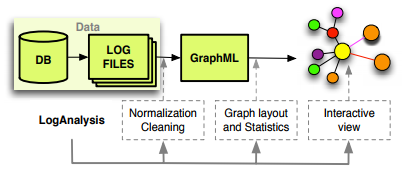
\includegraphics[width=\textwidth]{log_analyza}
	\caption{Architektúra \it{LogAnalysis}}
\end{figure}

Architektúra je tvorená rozšíriteľnými úrovňami: import dát vytvorenými informatívnymi
systémami mobilných telefónov (zvyčajne bytové súbory), konverzie do formátu GraphML, ktorý je štruktúrovaný formát XML vhodnejší pre grafické znázornenie a výmeny medzi aplikáciami na kreslenie grafov.

Cieľom je získať zaujímavé informácie pre vyšetrovanie z celkovej štruktúry siete.
 % viz. obsah.tex / see obsah.tex

  % Pouzita literatura / Bibliography
  % ----------------------------------------------
\ifslovak
  \makeatletter
  \def\@openbib@code{\addcontentsline{toc}{chapter}{Literatúra}}
  \makeatother
  \bibliographystyle{bib-styles/czechiso}
\else
  \ifczech
    \makeatletter
    \def\@openbib@code{\addcontentsline{toc}{chapter}{Literatura}}
    \makeatother
    \bibliographystyle{bib-styles/czechiso}
  \else 
    \makeatletter
    \def\@openbib@code{\addcontentsline{toc}{chapter}{Bibliography}}
    \makeatother
    \bibliographystyle{bib-styles/englishiso}
  %  \bibliographystyle{alpha}
  \fi
\fi
  \begin{flushleft}
  \bibliography{manual-20-literatura-bibliography}
  \end{flushleft}

  % vynechani stranky v oboustrannem rezimu
  % Skip the page in the two-sided mode
  \iftwoside
    \cleardoublepage
  \fi

  % Prilohy / Appendices
  % ---------------------------------------------
  \appendix
\ifczech
  \renewcommand{\appendixpagename}{Přílohy}
  \renewcommand{\appendixtocname}{Přílohy}
  \renewcommand{\appendixname}{Příloha}
\fi
\ifslovak
  \renewcommand{\appendixpagename}{Prílohy}
  \renewcommand{\appendixtocname}{Prílohy}
  \renewcommand{\appendixname}{Príloha}
\fi

% vynechani stranky v oboustrannem rezimu
% Skip the page in the two-sided mode
\iftwoside
  \cleardoublepage
\fi
  
\ifslovak
%  \section*{Zoznam príloh}
%  \addcontentsline{toc}{section}{Zoznam príloh}
\else
  \ifczech
%    \section*{Seznam příloh}
%    \addcontentsline{toc}{section}{Seznam příloh}
  \else
%    \section*{List of Appendices}
%    \addcontentsline{toc}{section}{List of Appendices}
  \fi
\fi
  \startcontents[chapters]
  % seznam příloh / list of appendices
  % \printcontents[chapters]{l}{0}{\setcounter{tocdepth}{2}}
  
  % vynechani stranky v oboustrannem rezimu
  \iftwoside
    \cleardoublepage
  \fi
  % % Tento soubor nahraďte vlastním souborem s přílohami (nadpisy níže jsou pouze pro příklad)
% This file should be replaced with your file with an appendices (headings below are examples only)

% Umístění obsahu paměťového média do příloh je vhodné konzultovat s vedoucím
% Placing of table of contents of the memory media here should be consulted with a supervisor
%\chapter{Obsah přiloženého paměťového média}

%\chapter{Manuál}

%\chapter{Konfigurační soubor} % Configuration file

%\chapter{RelaxNG Schéma konfiguračního souboru} % Scheme of RelaxNG configuration file

%\chapter{Plakát} % poster

\chapter{Jak pracovat s touto šablonou}
\label{jak}

V této kapitole je uveden popis jednotlivých částí šablony, po kterém následuje stručný návod, jak s touto šablonou pracovat. 

Jedná se o přechodnou verzi šablony. Nová verze bude zveřejněna do konce roku 2016 a bude navíc obsahovat nové pokyny ke správnému využití šablony, závazné pokyny k~vypracování bakalářských a diplomových prací (rekapitulace pokynů, které jsou dostupné na~webu) a nezávazná doporučení od vybraných vedoucích. Jediné soubory, které se v nové verzi změní, budou projekt-01-kapitoly-chapters.tex a projekt-30-prilohy-appendices.tex, jejichž obsah každý student vymaže a nahradí vlastním. Šablonu lze tedy bez problémů využít i~v~současné verzi.

\section*{Popis částí šablony}

Po rozbalení šablony naleznete následující soubory a adresáře:
\begin{DESCRIPTION}
  \item [bib-styles] Styly literatury (viz níže). 
  \item [obrazky-figures] Adresář pro Vaše obrázky. Nyní obsahuje placeholder.pdf (tzv. TODO obrázek, který lze použít jako pomůcku při tvorbě technické zprávy), který se s prací neodevzdává. Název adresáře je vhodné zkrátit, aby byl jen ve zvoleném jazyce.
  \item [template-fig] Obrázky šablony (znak VUT).
  \item [fitthesis.cls] Šablona (definice vzhledu).
  \item [Makefile] Makefile pro překlad, počítání normostran, sbalení apod. (viz níže).
  \item [projekt-01-kapitoly-chapters.tex] Soubor pro Váš text (obsah nahraďte).
  \item [projekt-20-literatura-bibliography.bib] Seznam literatury (viz níže).
  \item [projekt-30-prilohy-appendices.tex] Soubor pro přílohy (obsah nahraďte).
  \item [projekt.tex] Hlavní soubor práce -- definice formálních částí.
\end{DESCRIPTION}

Výchozí styl literatury (czechiso) je od Ing. Martínka, přičemž anglická verze (englishiso) je jeho překladem s drobnými modifikacemi. Oproti normě jsou v něm určité odlišnosti, ale na FIT je dlouhodobě akceptován. Alternativně můžete využít styl od Ing. Radima Loskota nebo od Ing. Radka Pyšného\footnote{BP Ing. Radka Pyšného \url{http://www.fit.vutbr.cz/study/DP/BP.php?id=7848}}. Alternativní styly obsahují určitá vylepšení, ale zatím nebyly řádně otestovány větším množstvím uživatelů. Lze je považovat za beta verze pro zájemce, kteří svoji práci chtějí mít dokonalou do detailů a neváhají si nastudovat detaily správného formátování citací, aby si mohli ověřit, že je vysázený výsledek v pořádku.

Makefile kromě překladu do PDF nabízí i další funkce:
\begin{itemize}
  \item přejmenování souborů (viz níže),
  \item počítání normostran,
  \item spuštění vlny pro doplnění nezlomitelných mezer,
  \item sbalení výsledku pro odeslání vedoucímu ke kontrole (zkontrolujte, zda sbalí všechny Vámi přidané soubory, a případně doplňte).
\end{itemize}

Nezapomeňte, že vlna neřeší všechny nezlomitelné mezery. Vždy je třeba manuální kontrola, zda na konci řádku nezůstalo něco nevhodného -- viz Internetová jazyková příručka\footnote{Internetová jazyková příručka \url{http://prirucka.ujc.cas.cz/?id=880}}.

\paragraph {Pozor na číslování stránek!} Pokud má obsah 2 strany a na 2. jsou jen \uv{Přílohy} a~\uv{Seznam příloh} (ale žádná příloha tam není), z nějakého důvodu se posune číslování stránek o 1 (obsah \uv{nesedí}). Stejný efekt má, když je na 2. či 3. stránce obsahu jen \uv{Literatura} a~je možné, že tohoto problému lze dosáhnout i jinak. Řešení je několik (od~úpravy obsahu, přes nastavení počítadla až po sofistikovanější metody). \textbf{Před odevzdáním proto vždy překontrolujte číslování stran!}


\section*{Doporučený postup práce se šablonou}

\begin{enumerate}
  \item \textbf{Zkontrolujte, zda máte aktuální verzi šablony.} Máte-li šablonu z předchozího roku, na stránkách fakulty již může být novější verze šablony s~aktualizovanými informacemi, opravenými chybami apod.
  \item \textbf{Zvolte si jazyk}, ve kterém budete psát svoji technickou zprávu (česky, slovensky nebo anglicky) a svoji volbu konzultujte s vedoucím práce (nebyla-li dohodnuta předem). Pokud Vámi zvoleným jazykem technické zprávy není čeština, nastavte příslušný parametr šablony v souboru projekt.tex (např.: \verb|documentclass[english]{fitthesis}| a přeložte prohlášení a poděkování do~angličtiny či slovenštiny.
  \item \textbf{Přejmenujte soubory.} Po rozbalení je v šabloně soubor projekt.tex. Pokud jej přeložíte, vznikne PDF s technickou zprávou pojmenované projekt.pdf. Když vedoucímu více studentů pošle projekt.pdf ke kontrole, musí je pracně přejmenovávat. Proto je vždy vhodné tento soubor přejmenovat tak, aby obsahoval Váš login a (případně zkrácené) téma práce. Vyhněte se však použití mezer, diakritiky a speciálních znaků. Vhodný název tedy může být např.: \uv{xlogin00-Cisteni-a-extrakce-textu.tex}. K přejmenování můžete využít i přiložený Makefile:
\begin{verbatim}
make rename NAME=xlogin00-Cisteni-a-extrakce-textu
\end{verbatim}
  \item Vyplňte požadované položky v souboru, který byl původně pojmenován projekt.tex, tedy typ, rok (odevzdání), název práce, svoje jméno, ústav (dle zadání), tituly a~jméno vedoucího, abstrakt, klíčová slova a další formální náležitosti.
  \item Nahraďte obsah souborů s kapitolami práce, literaturou a přílohami obsahem svojí technické zprávy. Jednotlivé přílohy či kapitoly práce může být výhodné uložit do~samostatných souborů -- rozhodnete-li se pro toto řešení, je doporučeno zachovat konvenci pro názvy souborů, přičemž za číslem bude následovat název kapitoly. 
  \item Nepotřebujete-li přílohy, zakomentujte příslušnou část v projekt.tex a příslušný soubor vyprázdněte či smažte. Nesnažte se prosím vymyslet nějakou neúčelnou přílohu jen proto, aby daný soubor bylo čím naplnit. Vhodnou přílohou může být obsah přiloženého paměťového média.
  \item Nascanované zadání uložte do souboru zadani.pdf a povolte jeho vložení do práce parametrem šablony v projekt.tex (\verb|documentclass[zadani]{fitthesis}|).
  \item Nechcete-li odkazy tisknout barevně (tedy červený obsah -- bez konzultace s vedoucím nedoporučuji), budete pro tisk vytvářet druhé PDF s tím, že nastavíte parametr šablony pro tisk: (\verb|documentclass[zadani,print]{fitthesis}|).  Barevné logo se nesmí tisknout černobíle!
  \item Vzor desek, do kterých bude práce vyvázána, si vygenerujte v informačním systému fakulty u zadání. Pro disertační práci lze zapnout parametrem v šabloně (více naleznete v souboru fitthesis.cls).
  \item Nezapomeňte, že zdrojové soubory i (obě verze) PDF musíte odevzdat na CD či jiném médiu přiloženém k technické zprávě.
\end{enumerate}

\subsection*{Pokyny pro oboustranný tisk}
\begin{itemize}
\item Zapíná se parametrem šablony: \verb|\documentclass[twoside]{fitthesis}|
\item Po vytištění oboustranného listu zkontrolujte, zda je při prosvícení sazební obrazec na obou stranách na stejné pozici. Méně kvalitní tiskárny s duplexní jednotkou mají často posun o 1--3 mm. Toto může být u některých tiskáren řešitelné tak, že vytisknete nejprve liché stránky, pak je dáte do stejného zásobníku a vytisknete sudé.
\item Za titulním listem, obsahem, literaturou, úvodním listem příloh, seznamem příloh a případnými dalšími seznamy je třeba nechat volnou stránku, aby následující část začínala na liché stránce (\textbackslash cleardoublepage).
\item  Konečný výsledek je nutné pečlivě překontrolovat.
\end{itemize}


\subsection*{Užitečné nástroje}
\label{nastroje}

Následující seznam není výčtem všech využitelných nástrojů. Máte-li vyzkoušený osvědčený nástroj, neváhejte jej využít. Pokud však nevíte, který nástroj si zvolit, můžete zvážit některý z následujících:

\begin{description}
	\item[\href{http://miktex.org/download}{MikTeX}] \LaTeX{} pro Windows -- distribuce s jednoduchou instalací a vynikající automatizací stahování balíčků.
	\item[\href{http://texstudio.sourceforge.net/}{TeXstudio}] Přenositelné opensource GUI pro \LaTeX{}.  Ctrl+klik umožňuje přepínat mezi zdrojovým textem a PDF. Má integrovanou kontrolu pravopisu, zvýraznění syntaxe apod. Pro jeho využití je nejprve potřeba nainstalovat MikTeX.
	\item[\href{http://jabref.sourceforge.net/download.php}{JabRef}] Pěkný a jednoduchý program v Javě pro správu souborů s bibliografií (literaturou). Není potřeba se nic učit -- poskytuje jednoduché okno a formulář pro editaci položek.
	\item[\href{https://inkscape.org/en/download/}{InkScape}] Přenositelný opensource editor vektorové grafiky (SVG i PDF). Vynikající nástroj pro tvorbu obrázků do odborného textu. Jeho ovládnutí je obtížnější, ale výsledky stojí za to.
	\item[\href{https://git-scm.com/}{GIT}] Vynikající pro týmovou spolupráci na projektech, ale může výrazně pomoci i jednomu autorovi. Umožňuje jednoduché verzování, zálohování a přenášení mezi více počítači.
	\item[\href{http://www.overleaf.com/}{Overleaf}] Online nástroj pro \LaTeX{}. Přímo zobrazuje náhled a umožňuje jednoduchou spolupráci (vedoucí může průběžně sledovat psaní práce), vyhledávání ve zdrojovém textu kliknutím do PDF, kontrolu pravopisu apod. Zdarma jej však lze využít pouze s určitými omezeními (někomu stačí na disertaci, jiný na ně může narazit i při psaní bakalářské práce) a pro dlouhé texty je pomalejší.
\end{description}

\subsection*{Užitečné balíčky pro \LaTeX}

Studenti při sazbě textu často řeší stejné problémy. Některé z nich lze vyřešit následujícími balíčky pro \LaTeX:

\begin{itemize}
  \item \verb|amsmath| -- rozšířené možnosti sazby rovnic,
  \item \verb|float, afterpage, placeins| -- úprava umístění obrázků,
  \item \verb|fancyvrb, alltt| -- úpravy vlastností prostředí Verbatim, 
  \item \verb|makecell| -- rozšíření možností tabulek,
  \item \verb|pdflscape, rotating| -- natočení stránky o 90 stupňů (pro obrázek či tabulku),
  \item \verb|hyphenat| -- úpravy dělení slov,
  \item \verb|picture, epic, eepic| -- přímé kreslení obrázků.
\end{itemize}

Některé balíčky jsou využity přímo v šabloně (v dolní části souboru fitthesis.cls). Nahlédnutí do jejich dokumentace může být rovněž užitečné.

Sloupec tabulky zarovnaný vlevo s pevnou šířkou je v šabloně definovaný \uv{L} (používá se jako \uv{p}).

 % viz. prilohy.tex / see prilohy.tex
\end{document}
